\section{Experiment Design}

To ensure experimental validity, all intermediate evaluation and hyperparameter tuning was performed on $23$ randomly selected images that were separate from both the training image set of $106$ images and the final test set of $23$ images. This split generated $27,623$ glyph images for training with $7,759$ glyph images being available for evaluation and $6,835$ glyph images for testing. All examples and images, and some intermediate evaluations, are taken from the evaluation set, with final metrics being taken on the test set. No results are taken from the training set, as they would have little meaning.

\section{Existing Pipelines}

To attempt to generate a baseline to assess new methods against, Tesseract \cite{SmithTesseract}, a popular OCR engine sponsored by Google \cite{Vincent} and Ocular \cite{Berg-Kirkpatrick}, another OCR engine based on stochastic models, were integrated into the pipeline using Pytesseract \cite{Lee} and by calling jar files from python respectively.

\subsection{Evaluation Metrics}

As these existing pipelines were assessed in the early phases of the project, a full ground truth to evaluate them on was not yet generated as the bounding of lines was not fully implemented. Therefore, they were assessed on how well they were able to detect the quantity of glyphs in an image and how visually close the transcriptions looked when the images were looked at by a human. These metrics proved to be enough to evaluate the methods as both methods were far enough away from an acceptable solution that a more exact metric for comparison was not needed.

\subsection{Tesseract}

With Tesseract, using the ancient Greek corpus, and using both raw and binarized images, the output was comparable to noise, with the transcription lengths being an order of magnitude different from the ground truths.

\subsection{Ocular}

Similarly, training Ocular on both raw and binarized full images and individual glyph images, the output was comparable to noise, with the transcription lengths being an order of magnitude different from the ground truths and $A$ and $\Lambda$ making up over $95\%$ of the returned glyphs. This result happened regardless of the dataset that Ocular was trained on, with binarized and non-binarized images performing the same and singular glyph images performing the same as whole images.

\section{Binarization}

\subsection{Evaluation Metrics}
As there was no ground-truth information provided to compare binarizations against, visual comparison was utilized to determine which binarization method was providing the highest quality binarizations. Evaluation was performed on four different images, which contained various features that would allow for quick visual evidence of the effectiveness of the methods \seefig{binarizationRaw}. Images from the training image set were utilized in hyperparameter optimization for the binarization methods, which included generating binarizations of more than four images. The four images are of assorted sizes, from different collections, and are degraded to different degrees, allowing them to function as a valuable quick assessment tool without introducing bias into the evaluation of the methods using visually approximated signal-to-noise ratio as a metric.

To assess each binarization method, these images, containing a total of approximately $300$ glyphs, were used to determine how much of the ink on the papyrus was being included, and if noise was being added to the image in the form of background pixels being black or ink pixels being white. This metric was designed to ensure that the signal-to-noise ratio would be low and that the recall and precision would be high, even if these metrics were not directly measurable without an expert-generated ground truth for each pixel.

\begin{figure}[H]
    \caption{Four Images Utilized to Visually Assess Binarization Quality}
    \label{fig:binarizationRaw}
    \begin{center}
        \begin{subfigure}[b]{0.45\textwidth}
            \centering
            \caption{Example File A}
            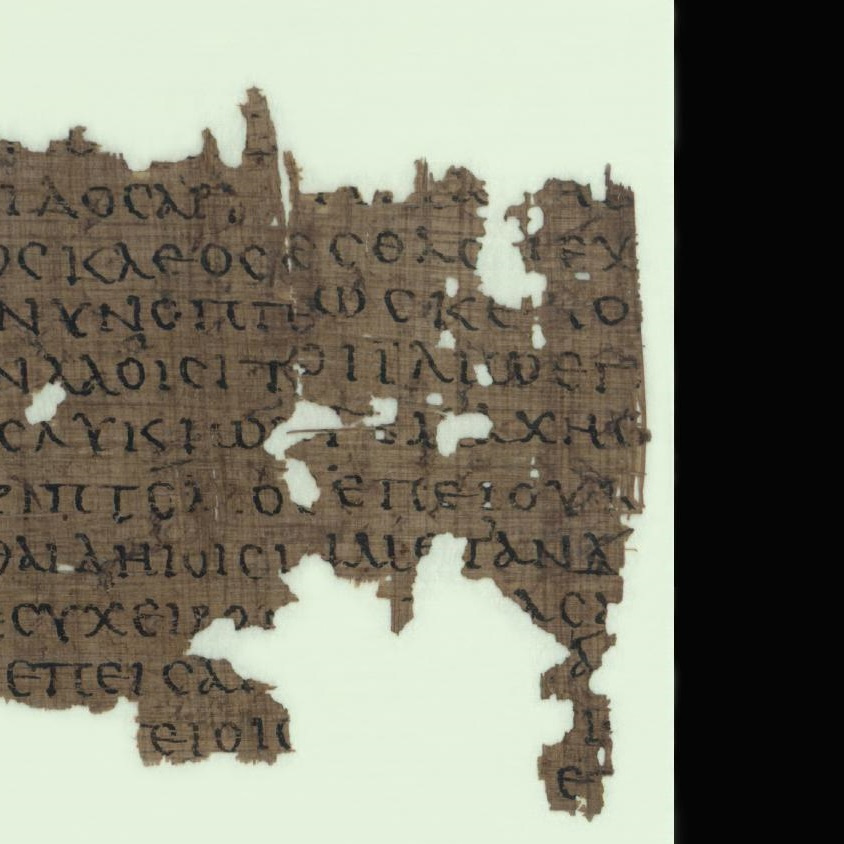
\includegraphics[width=\textwidth]{{raw/G_02317_26742_Pap_crop.jpg}}
        \end{subfigure}
        \hfill
        \begin{subfigure}[b]{0.45\textwidth}
            \centering
            \caption{Example File B}
            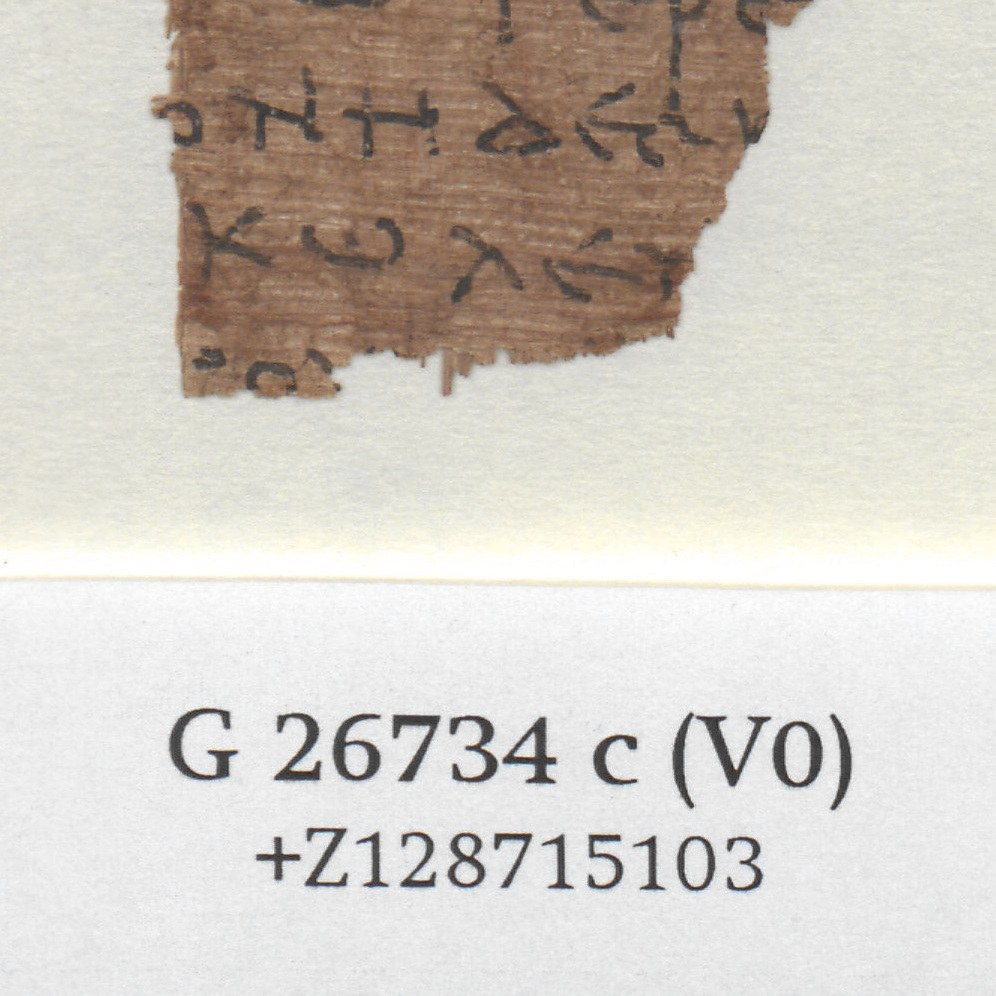
\includegraphics[width=\textwidth]{{raw/G_26734_c_crop.jpg}}
        \end{subfigure}
        \vfill
        \begin{subfigure}[b]{0.45\textwidth}
            \centering
            \caption{Example File C}
            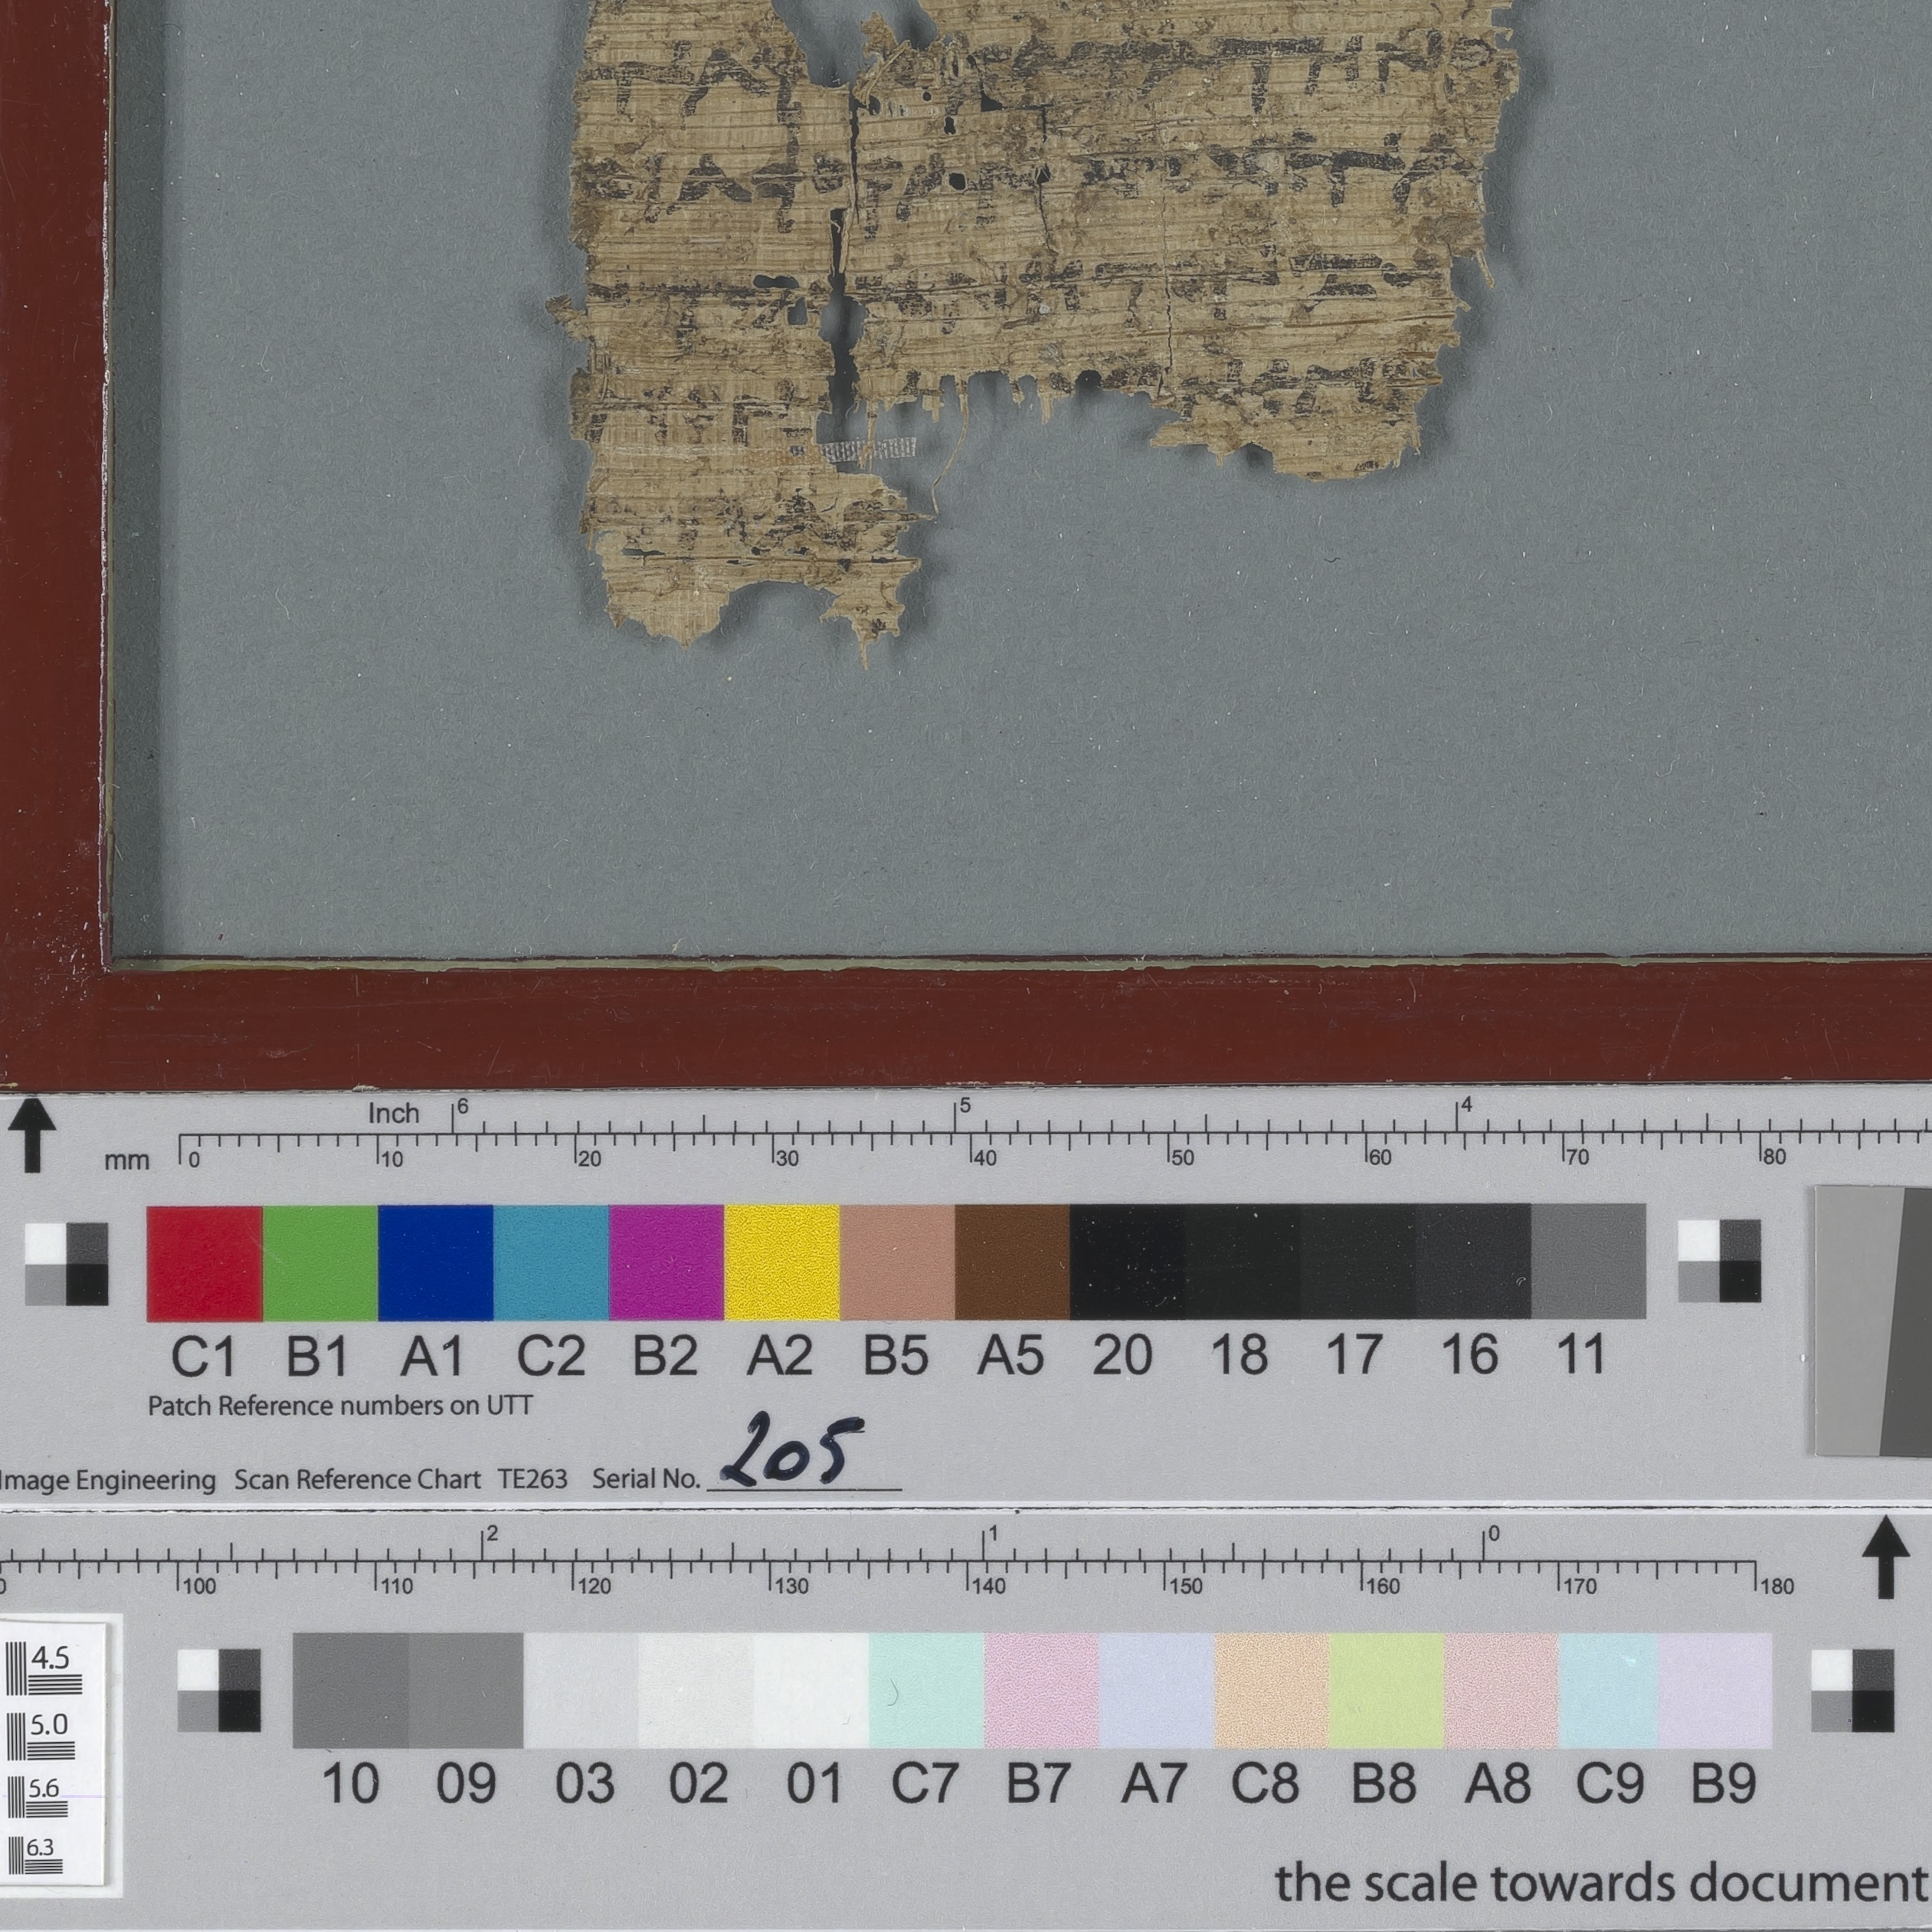
\includegraphics[width=\textwidth]{{raw/P_Hamb_graec_665_crop.jpg}}
        \end{subfigure}
        \hfill
        \begin{subfigure}[b]{0.45\textwidth}
            \centering
            \caption{Example File D}
            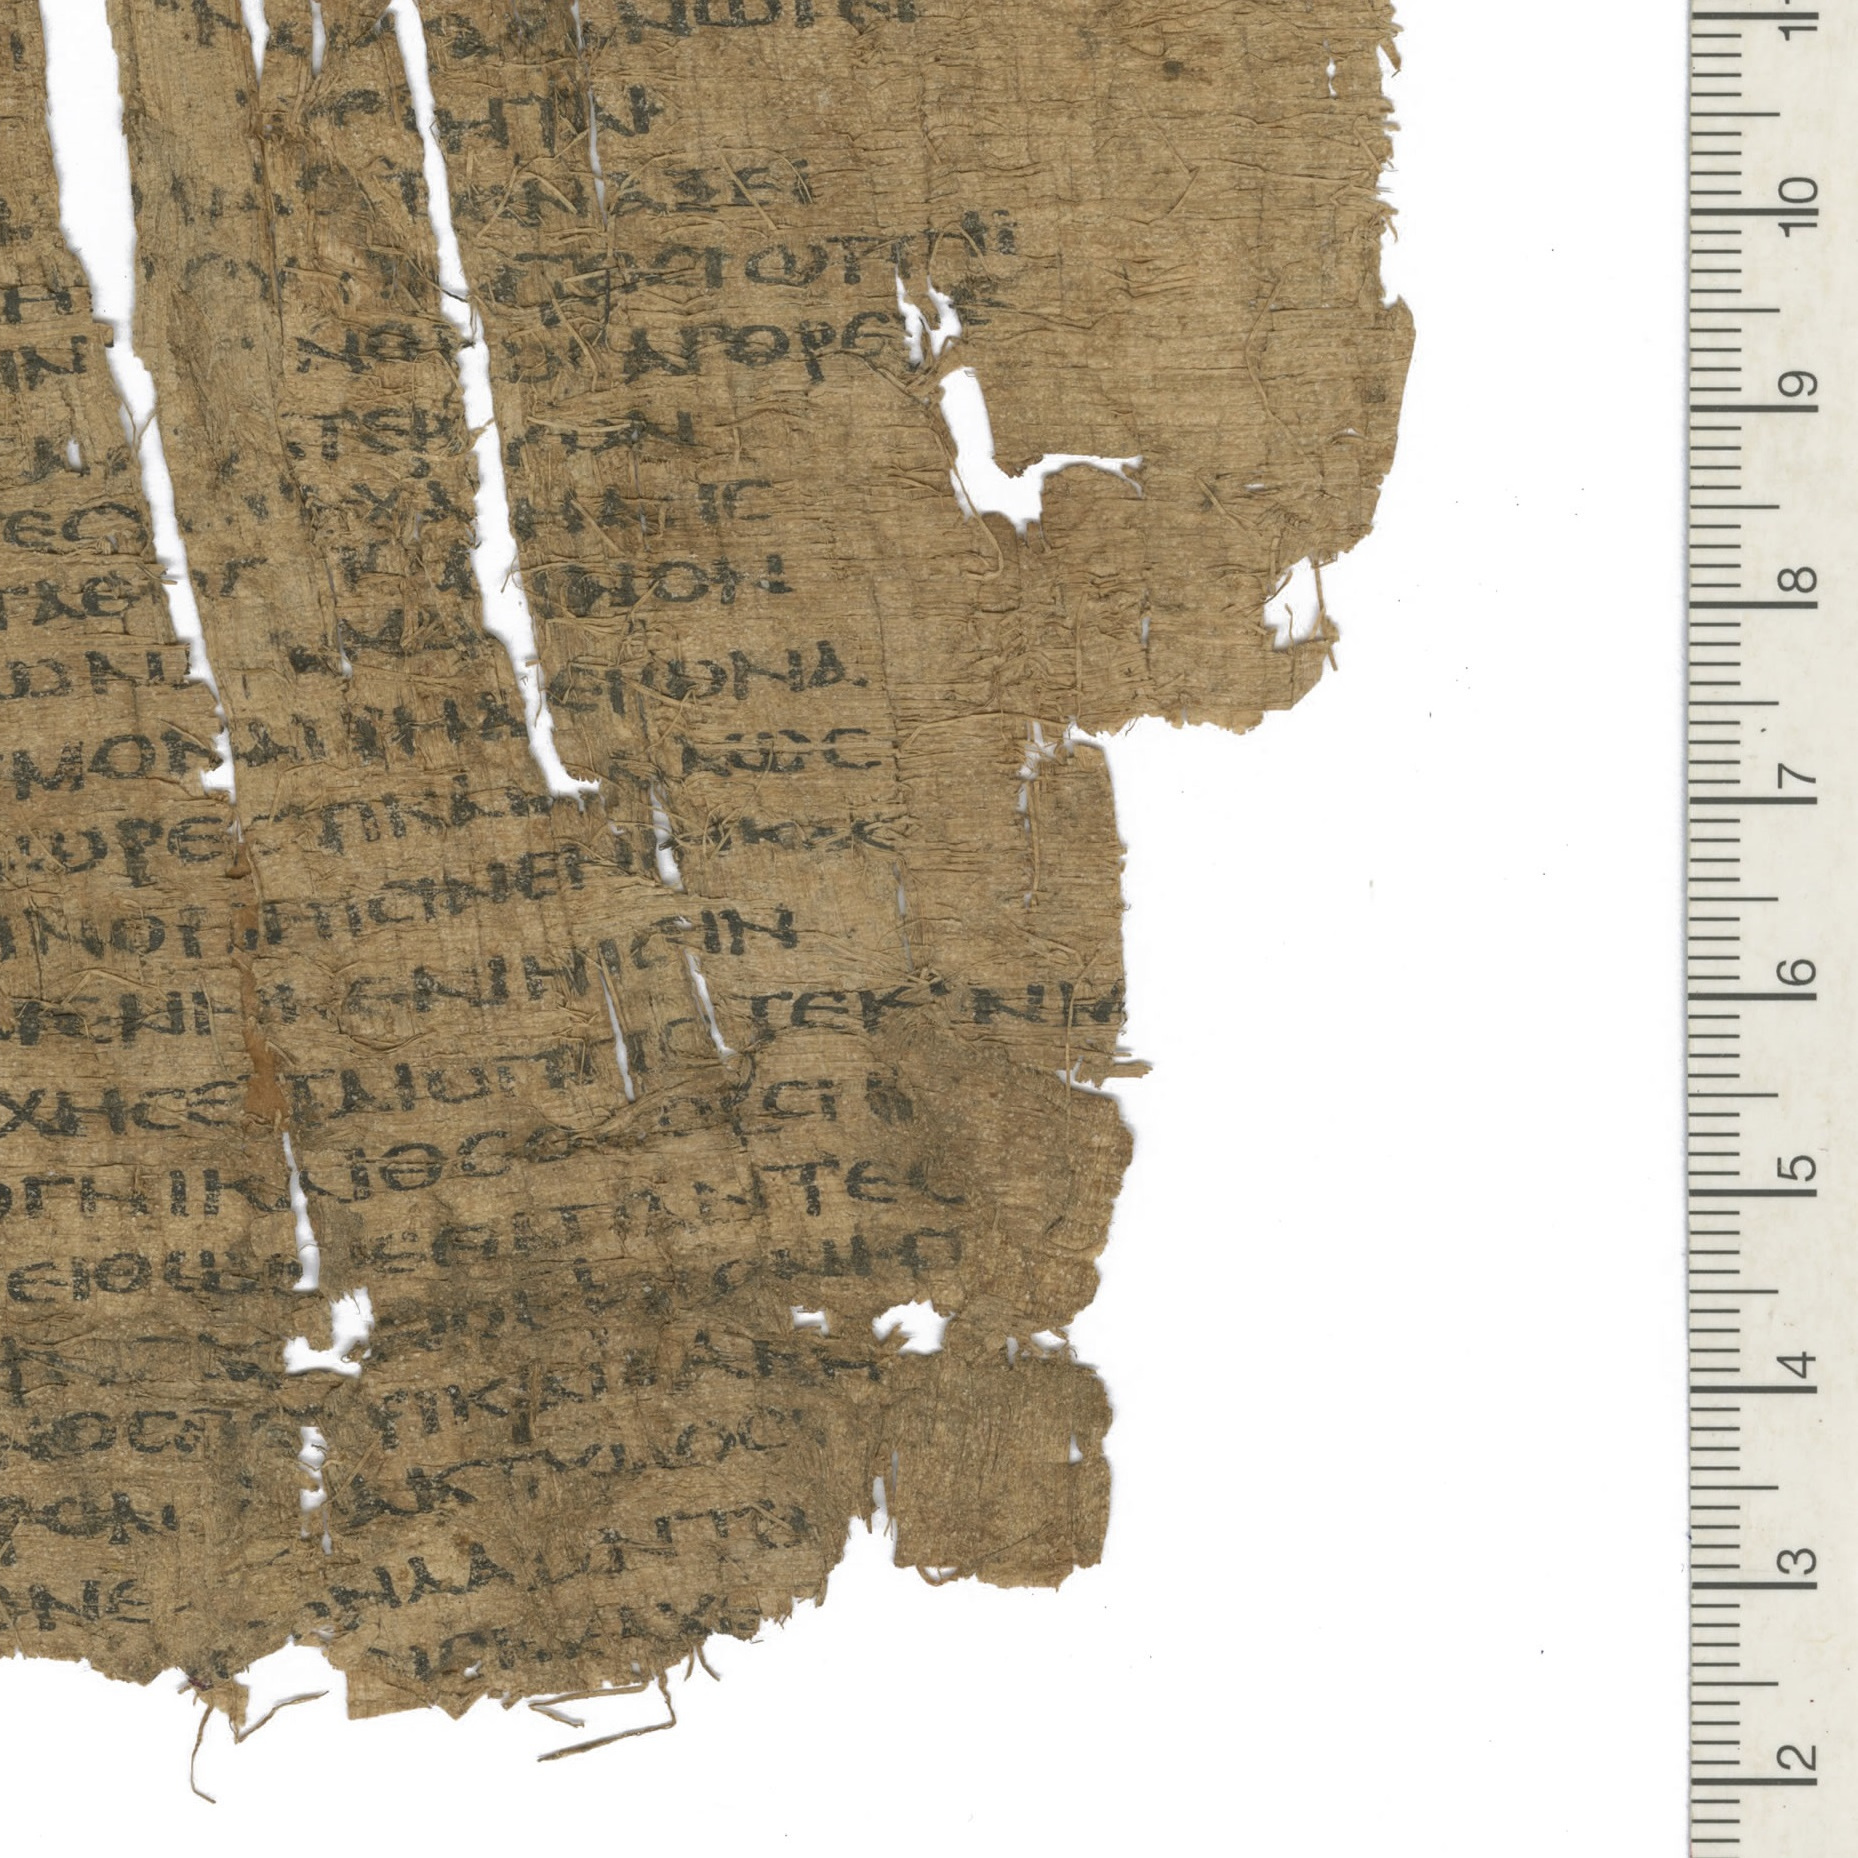
\includegraphics[width=\textwidth]{{raw/PSI_XIV_1377r_crop.jpg}}
        \end{subfigure}
    \end{center}
    The four images used to assess binarization methods, cropped to squares so that are easy to tile to make it easy to assess visually.
\end{figure}

\subsection{Evaluation of Methods}

The results of k-means clustering on the evaluation images are included for reference \seefig{binarizationClustering}. These images clearly show that the signal-to-noise ratio is far too high to be utilized as the general binarization solution for the pipeline, as the approximated signal-to-noise ratio is sometimes less than $1$, with significantly more noise than signal being generated.

The results generated by clustering can be directly compared to those of a neural network to see how poor they are. The results generated by DP-Linknet \seefig{binarizationCNN} are visibly much better at including whole glyphs and less of the noise included in the image, especially the papyrus noise.

Using the results of the Gabor wavelet approximation \seefig{binarizationGabor}, a binary mask can be created \seefig{binarizationGaborBinary} using DP-Linknet. This works using the assumption that large amounts of noise in the binary images generated by DP-Linknet are due to intentionally added objects in the original images, which are often more regular in color or shape than the glyphs. This means the Gabor-filtered images do not lose this noise, allowing the CNN to pick up on this information to create an image that can be used as a mask to remove these details from the final binarizations \seefig{binarizationMaskedCNN}.

\begin{figure}[H]
    \caption{Four Example Binarizations Generated with Clustering}
    \label{fig:binarizationClustering}
    \begin{center}
        \begin{subfigure}[b]{0.45\textwidth}
            \centering
            \caption{Example File A}
            
\includegraphics[width=\textwidth]{{binarization/clustering/G_02317_26742_Pap_crop.png}}
        \end{subfigure}
        \hfill
        \begin{subfigure}[b]{0.45\textwidth}
            \centering
            \caption{Example File B}
            \includegraphics[width=\textwidth]{{binarization/clustering/G_26734_c_crop.png}}
        \end{subfigure}
        \vfill
        \begin{subfigure}[b]{0.45\textwidth}
            \centering
            \caption{Example File C}
            \includegraphics[width=\textwidth]{{binarization/clustering/P_Hamb_graec_665_crop.png}}
        \end{subfigure}
        \hfill
        \begin{subfigure}[b]{0.45\textwidth}
            \centering
            \caption{Example File D}
            \includegraphics[width=\textwidth]{{binarization/clustering/PSI_XIV_1377r_crop.png}}
        \end{subfigure}
    \end{center}
    The four images were used to assess binarization methods, binarized using k-means with $k=5$. Image A has a poor signal-to-noise ratio. Image B has a much better signal-to-noise ratio for the glyphs, but also contains text that should not be included near the bottom of the image. Images l and D also contain glyph-signal, but are both noisy around the glyphs and include non-glyph information such as a ruler in Image D and the border and color scale in image C.
\end{figure}

\begin{figure}[H]
    \caption{Four Example Binarizations Generated with DP-Linknet}
    \label{fig:binarizationCNN}
    \begin{center}
        \begin{subfigure}[b]{0.45\textwidth}
            \centering
            \caption{Example File A}
            
\includegraphics[width=\textwidth]{{binarization/cnn/G_02317_26742_Pap_crop.png}}
        \end{subfigure}
        \hfill
        \begin{subfigure}[b]{0.45\textwidth}
            \centering
            \caption{Example File B}
            \includegraphics[width=\textwidth]{{binarization/cnn/G_26734_c_crop.png}}
        \end{subfigure}
        \vfill
        \begin{subfigure}[b]{0.45\textwidth}
            \centering
            \caption{Example File C}
            \includegraphics[width=\textwidth]{{binarization/cnn/P_Hamb_graec_665_crop.png}}
        \end{subfigure}
        \hfill
        \begin{subfigure}[b]{0.45\textwidth}
            \centering
            \caption{Example File D}
            \includegraphics[width=\textwidth]{{binarization/cnn/PSI_XIV_1377r_crop.png}}
        \end{subfigure}
    \end{center}
    The four images used to assess binarization methods, binarized using DP-Linknet \cite{Xiong} with  confidence value of 2. Image A has clearly defined glyphs, especially when compared to the results of clustering. Image B has a similar signal-to-noise ratio for the glyphs to the clustering, with the extra text near the bottom of the image still being included. Images l and D also contain glyph-signal, and are less noisy around the glyphs and include non-glyph information such as a ruler in Image D and the border and color scale in image C.
\end{figure}

\begin{figure}[H]
    \caption{Four Example Gabor-Filtered Images}
    \label{fig:binarizationGabor}
    \begin{center}
        \begin{subfigure}[b]{0.45\textwidth}
            \centering
            \caption{Example File A}
            
\includegraphics[width=\textwidth]{{binarization/gabor/G_02317_26742_Pap_crop.png}}
        \end{subfigure}
        \hfill
        \begin{subfigure}[b]{0.45\textwidth}
            \centering
            \caption{Example File B}
            \includegraphics[width=\textwidth]{{binarization/gabor/G_26734_c_crop.png}}
        \end{subfigure}
        \vfill
        \begin{subfigure}[b]{0.45\textwidth}
            \centering
            \caption{Example File C}
            \includegraphics[width=\textwidth]{{binarization/gabor/P_Hamb_graec_665_crop.png}}
        \end{subfigure}
        \hfill
        \begin{subfigure}[b]{0.45\textwidth}
            \centering
            \caption{Example File D}
            \includegraphics[width=\textwidth]{{binarization/gabor/PSI_XIV_1377r_crop.png}}
        \end{subfigure}
    \end{center}
    The four images used to assess binarization methods, passed through the Gabor wavelet approximation function.
\end{figure}

\begin{figure}[H]
    \caption{Four Example Gabor Wavelet Binarized Images}
    \label{fig:binarizationGaborBinary}
    \begin{center}
        \begin{subfigure}[b]{0.45\textwidth}
            \centering
            \caption{Example File A}
            
\includegraphics[width=\textwidth]{{binarization/gaborMask/G_02317_26742_Pap_crop.png}}
        \end{subfigure}
        \hfill
        \begin{subfigure}[b]{0.45\textwidth}
            \centering
            \caption{Example File B}
            \includegraphics[width=\textwidth]{{binarization/gaborMask/G_26734_c_crop.png}}
        \end{subfigure}
        \vfill
        \begin{subfigure}[b]{0.45\textwidth}
            \centering
            \caption{Example File C}
            \includegraphics[width=\textwidth]{{binarization/gaborMask/P_Hamb_graec_665_crop.png}}
        \end{subfigure}
        \hfill
        \begin{subfigure}[b]{0.45\textwidth}
            \centering
            \caption{Example File D}
            \includegraphics[width=\textwidth]{{binarization/gaborMask/PSI_XIV_1377r_crop.png}}
        \end{subfigure}
    \end{center}
    The four images used to assess binarization methods, passed through the Gabor wavelet approximation function and then passed through DP-Linknet to create a rudimentary mask that contains some non-glyph information.
\end{figure}

\begin{figure}[H]
    \caption{Four Example CNN Binarized Images (Masked)}
    \label{fig:binarizationMaskedCNN}
    \begin{center}
        \begin{subfigure}[b]{0.45\textwidth}
            \centering
            \caption{Example File A}
            
\includegraphics[width=\textwidth]{{binarization/cnnMasked/G_02317_26742_Pap_crop.png}}
        \end{subfigure}
        \hfill
        \begin{subfigure}[b]{0.45\textwidth}
            \centering
            \caption{Example File B}
            \includegraphics[width=\textwidth]{{binarization/cnnMasked/G_26734_c_crop.png}}
        \end{subfigure}
        \vfill
        \begin{subfigure}[b]{0.45\textwidth}
            \centering
            \caption{Example File C}
            \includegraphics[width=\textwidth]{{binarization/cnnMasked/P_Hamb_graec_665_crop.png}}
        \end{subfigure}
        \hfill
        \begin{subfigure}[b]{0.45\textwidth}
            \centering
            \caption{Example File D}
            \includegraphics[width=\textwidth]{{binarization/cnnMasked/PSI_XIV_1377r_crop.png}}
        \end{subfigure}
    \end{center}
    The four images used to assess binarization methods, binarized using DP-Linknet \cite{Xiong} with  confidence value of 2 and then masked by the binarizations of the Gabor-filtered images with the removed black parts of the image shown in grey. No changes were made to image A, as there was no detail that the CNN could recognize left in the Gabor-filtered image. The extra text from image B is mostly removed, with the glyph information intact. Similarly, images l and D have their glyph information intact, with the artificial noise in the image being partially removed.
\end{figure}

\section{Glyph Bounding}

\subsection{Evaluation Metrics}

As the ground-truth information provided for bounding boxes is not tight, perfectly accurate metrics on bounding are not possible without manually tightly rebounding each glyph. Therefore, IOU is used, along with glyph precision and recall measuring the approximate efficacy of methods, with the caveat that a method may have a lower IOU if it generates tighter bounding boxes than if the bounding box was less tight.

Precision and recall are measured on glyphs, ignoring the exact pixels and sizes of the bounding boxes. A prediction is defined as a match for a known bounding box if the IOU between the two bounding boxes is greater than zero. Each ground truth bounding box is then paired with the matched prediction bounding box with the highest IOU value such that no bounding box is paired with more than one other bounding box. The mean IOU is also recorded for all true positives as a method to determine how close the prediction bounding boxes are to the ground truth values.

\begin{figure}[H]
    \caption{Test Results for Glyph Bounding Methods}
    \label{fig:boundingEval}
    \centering
    \begin{tabular}{ | l | l | l | l | l | }
        \hline
        Bounding Method & Precision & Recall & F1 Score & Mean IOU \\
        \hline
        Connected Components (CC) & 0.2006 & 0.8923 & 0.3276 & 0.3182 \\
        CC w/ Best Cleaning & 0.2335 & 0.8093 & 0.3624 & 0.3142 \\
        \hline
    \end{tabular}
\end{figure}

\subsection{Connected Components}

Glyph bounding using connected components fails to precisely generate bounding boxes due to the flaws in the binarization methods used. Otherwise, the method can tightly bound boxes with a high amount of recall. By removing regions with centroids in other regions or by removing regions fully inside other regions (which includes the before method), the precision and F1 score can be increased, at the cost of recall \seefig{ccBoundingEval}.

\begin{figure}[H]
    \caption{Test Results for Connected Component Bounding and Cleaning}
    \label{fig:ccBoundingEval}
    \centering
    \begin{tabular}{ | l | l | l | l | l | }
        \hline
        Cleaning Method & Precision & Recall & F1 Score & Mean IOU \\
        \hline
        None & 0.2006 & 0.8923 & 0.3276 & 0.3182 \\
        Internal Centroid Removal & 0.2256 & 0.8124 & 0.3531 & 0.3145 \\
        Internal Region Removal & 0.2335 & 0.8093 & 0.3624 & 0.3142 \\
        \hline
    \end{tabular}
\end{figure}

\subsection{Region-Based Convolution Neural Networks}

YOLO, when trained on color images, performs better than when trained on binarized images. In addition, by training YOLO to recognize all glyphs as one class instead of each glyph class as its own class the accuracy can be significantly increased \seefig{evalYOLORaw}. In addition, networks were trained with and without freezing the backbone layers, which are the layers defined as the initial convolutional layers (layers 0-9) \cite{YOLOBackbone} that process the input before the main convolutions are performed. This allowed for faster training with a potential for lost accuracy.

\textit{The accuracy metrics taken for each YOLO model were generated on the evaluation set to ensure that the final test set evaluation could be done on unseen data. Therefore, the classification metrics in this sub-section will not map directly to the results of the same classification methods when utilized in the final pipeline.}

\begin{figure}[H]
    \caption{Evaluation Results for YOLO Bounding}
    \label{fig:evalYOLORaw}
    \begin{center}
      \begin{tabular}{ | l | l | l | l | l | }
          \hline
          Training Set & Backbone Layers & Image Type & Model Size & F1 Score \\
          \hline
          Multi-Class & Frozen & Color & YOLOv5x (largest) & 0.07 \\
          Mono-Class & Frozen & Binary & YOLOv5l (large) & 0.63 \\
          Mono-Class & Frozen & Color & YOLOv5l (large) & 0.68 \\
          Mono-Class & Frozen & Color & YOLOv5x (largest) & 0.69 \\
          Mono-Class & Unfrozen & Color & YOLOv5x (largest) & 0.74 \\
          Mono-Class & Unfrozen & Color & YOLOv5x (largest) & 0.72* \\
          \hline
      \end{tabular}
    \end{center}
    \vspace{5mm}
    All the models were trained for 300 epochs, with the exception of the Model with a * next to the F1 score, which was trained for 600 epochs, with the F1 score being taken on only the last 300 epochs.
\end{figure}

\subsubsection{RCCN Sliding Window}

By using the model with the highest base F1 score and introducing a sliding window to the RCNN, the peak F1 score can be increased. This effect is amplified by introducing an inner sliding window, which reduces the recall for the benefit of more precision \seefig{evalYOLOSliding}.

\begin{figure}[H]
    \caption{Evaluation Results for Sliding Window Assisted YOLO Bounding}
    \label{fig:evalYOLOSliding}
    \begin{center}
      \begin{tabular}{ | l | l | l | l | l | }
          \hline
          Inner Window & Type & Precision & Recall & F1 Score \\
          \hline
          False & Mean & 0.934 & 0.851 & 0.874 \\
          False & Max F1 Score & 0.926 & 0.936 & 0.931 \\
          True & Mean & 0.953	& 0.830 & 0.870 \\
          True & Max F1 Score & 0.929 & 0.942 & 0.936 \\
          \hline
      \end{tabular}
    \end{center}
    \vspace{5mm}
    All results are taken with a sliding window of $800$ pixels and a step size of $200$ pixels. The results are averaged over the confidence thresholds $t$ required for the bounding boxes to be kept, where $0.1 \leq t \leq .85$ with a step size of $.05$.
\end{figure}

\subsubsection{RCNN Duplicate Removal}
YOLO generates a confidence value for each bounding box. Using these confidence levels, ties between overlapping bounding boxes are broken where bounding boxes are defined as having an IOU above a threshold. Using this method to break ties, in addition to a minimum confidence level for bounding boxes, duplicates can be much more effectively removed, increasing the maximum F1 score of the bounding boxes \seefig{evalYOLODuplicates}.

\begin{figure}[H]
    \caption{Evaluation Results for Maximal F1 Score for Sliding Window Duplicate Removal}
    \label{fig:evalYOLODuplicates}
    \begin{center}
      \begin{tabular}{ | l | l | l | l | l | l | }
          \hline
          Inner Window & Confidence & Duplicate IOU & Precision & Recall & F1 Score \\
          \hline
          False & 0.47 & 0.33 & 0.940	& 0.928	& 0.934 \\
          True & 0.29	& 0.45 & 0.931 & 0.944 & 0.937 \\
          \hline
      \end{tabular}
    \end{center}
    \vspace{5mm}
    All results are taken with a sliding window of $800$ pixels and a step size of $200$ pixels. The maximum F1 score values were found by narrowing the hyperparameter search window and decreasing step size until the 3 significant figures of the F1 score no longer changed.
\end{figure}

\subsubsection{Binarization-Assisted CNN}
Using the binary images to tightly crop the YOLO-generated bounding boxes to the ink generates bounding boxes that have a mean IOU of $71.5\%$ compared to a mean IOU of $73.0\%$ without cropping the bounding boxes. This difference in bounding box size and shape results in a difference of less an a $.01\%$ in the mean precision, recall, and F1 scores. Cropping bounding boxes using the binarized images also reduces the mean classification F1 score by $1.8\%$.

\section{Line Bounding}

As in glyph bounding, no ground truth information was provided for which glyphs where in the same line, so a visual approximation must be used to determine which methods are best, at least when comparing results of each metric without taking the rest of the pipeline into account.

\subsection{Point-Of-Interest Clustering}

Using point-of-interest clustering fails to generate valid lines as the noise in both the binarized and color images preventing the glyphs from being clustered correctly, which causes higher frequency noise to be made into lines, instead of the glyphs. Given more time, the application of de-noising techniques could be explored to make this method more effective.

\subsection{Adjacent and Overlapping Glyph Clustering}

Grouping glyph bounding boxes into lines based on adjacency and overlapping produces significantly better results than would otherwise be generated, with this method improving the mean classification F1 score by $2.6\%$ on the best performing LSTM-based CNN classifier.

\subsection{Line-Based Bounding Box Cropping}

Using line-based bounding box cropping to prevent bounding boxes from overlapping has a negative effect on glyph classification accuracy, but a small positive effect on bounding accuracy \seefig{lineIntersect}. When combined with bounding box cropping, this effect is amplified, further reducing classification and bounding box accuracies.

\begin{figure}[H]
    \caption{Evaluation Results for Bounding Box Intersection Removal on Bounding Box and Classification F1 Scores}
    \label{fig:lineIntersect}
    \begin{center}
      \begin{tabular}{ | l | l | l | l | }
          \hline
          Intersection & Tight & Bounding Box & Classification \\
          Removed & Bounding Boxes & F1 Score & F1 Score \\
          \hline
          True & True & 0.872	& 0.797 \\
          True & False & 0.873 & 0.807 \\
          False & True & 0.872 & 0.805 \\
          False & False & 0.872	& 0.809 \\
          \hline
      \end{tabular}
    \end{center}
\end{figure}

\subsection{Line Variation Generation}

Using lines to generate bounding box variations produced negative results on both the bounding and classification accuracy of the pipeline \seefig{lineVariants}. Variations are made based on the likelihood of the classifications, which, depending on the classifier used, could lead to worse line variants being accepted over the original line. This is because partial glyphs, such as the two halves of a $\Pi$, may closely resemble and be classified as other glyphs, such as a $\Gamma$ and a $T$. If this happens, then the line variant with the split $\Pi$ could be considered more likely, especially if the $\Pi$ is poorly formed or has noise in the upper right corner, for example.

\begin{figure}[H]
    \caption{Evaluation Results for Line-Based Bounding Box Variation}
    \label{fig:lineVariants}
    \begin{center}
      \begin{tabular}{ | l | l | l | l | }
          \hline
          Line Variants & Bounding & Classification & Combined \\
          Generated & F1 Score & F1 Score & F1 Score \\
          \hline
          True & 0.885 & 0.795 & 0.707 \\
          False & 0.910 &	0.811 &	0.741 \\
          \hline
      \end{tabular}
    \end{center}
\end{figure}

\section{Classification}

\textit{The accuracy metrics taken for the classification methods were generated on the evaluation set to ensure that the final test set evaluation could be done on unseen data. Therefore, the classification metrics in this section will not map directly to the results of the same classification methods when utilized in the final pipeline.}

\subsection{Transfer Learning}

Using the feature vectors generated with AlexNet on the non-NN methods, the best results were obtained using the binarizations of the images generated by DP-Linknet. GMMs, Random Forests, and $K$-Nearest Neighbors (k-NN) classifiers were generated with the full color and binarized images and Euclidean distance calculations \seeeq{distanceEuclidian}, with the best results for each method being shown \seefig{classificationEuclideanNonNN}, where F1 score is the average of the per-glyph F1 score weighted by glyph class occurrence frequency.

\begin{figure}[H]
    \caption{Evaluation Results for Euclidean Non-NN Transfer Learning Classification}
    \label{fig:classificationEuclideanNonNN}
    \centering
    \begin{tabular}{ | l | l | l | }
        \hline
        Classification Method & Color F1 Score & Binary F1 Score \\
        \hline
        GMM & 0.07 & 0.08 \\
        Random Forest & 0.11 & 0.19 \\
        KNN & 0.08 & 0.14 \\
        \hline
    \end{tabular}
\end{figure}

By generating a new set of training data by training the classifications on exactly one randomly chosen template for each class and footmark type, the results were mostly unchanged, but were significantly increased by manually cleaning the templates to remove noise and other small imperfections in the characters \seefig{classificationKNNTemplates}. These results were generated using only a k-NN classifier as it was the fastest to train and did not require as many example images to train an accurate model. These results show that the k-NN classifier can be trained on very few images and generate comparable results to a dataset that is magnitudes larger, which shows promise for classification on similar problems with significantly less training data.

\begin{figure}[H]
    \caption{Evaluation Results for Templated k-NN Transfer Learning Classification}
    \label{fig:classificationKNNTemplates}
    \centering
    \begin{tabular}{ | l | l | l | l | }
        \hline
        Template Type & Distance & Best $k$ Value & Weighted F1 Score \\
        \hline
        Color & Euclidean & 5 & 0.08 \\
        Cleaned Binary & Euclidean & 5 & 0.27 \\
        Cleaned Binary & Manhattan & 4 & 0.34 \\
        Cleaned Binary & Cosine & 5 & 0.39 \\
        \hline
    \end{tabular}
\end{figure}

Using pretrained neural networks to classify the data generated better results, both on binarized and color images of glyphs \seefig{classificationFeatureVectorNN}. Using these networks a higher classification accuracy was attainable with unaltered training data, producing better results with less manual work being required.

\begin{figure}[H]
    \caption{Evaluation Results for NN Transfer Learning Classification}
    \label{fig:classificationFeatureVectorNN}
    \centering
    \begin{tabular}{ | l | l | l | }
        \hline
        Network & Image Type & Weighted F1 Score \\
        \hline
        Linear \ref{fig:nnLinear} & Binary & 0.666 \\
        Linear \ref{fig:nnLinear} & Color & 0.626 \\
        Simple-LSTM \ref{fig:nnSimpleLSTM} & Color & 0.593 \\
        LSTM-to-Linear \ref{fig:nnLinear2LSTM} & Color & 0.662 \\
        Linear-to-LSTM \ref{fig:nnLSTM2Linear} & Binary & 0.710 \\
        Linear-to-LSTM \ref{fig:nnLSTM2Linear} & Color & 0.668 \\
        \hline
    \end{tabular}
\end{figure}

\subsection{Convolutional Neural Networks}
By training the convolutional layers of AlexNet \cite{Krizhevsky}, ResNeXt \cite{Xie}, and MNIST9975 \cite{Deotte}, the accuracy of the classifiers were able to be further increased. The convolutional network based on AlexNet generates similar results to those generated by the classifiers based on the feature vectors generated by AlexNet, but has a higher weighted F1 score. The networks based on ResNeXt perform even better, at the cost of time, taking much longer to train and evaluate \seefig{classificationCNN}. In these larger, more complex models, the binarized images performed worse than the color images across all the models, so only the peak color image F1 score is used for evaluation. Each network was trained and evaluated for approximately $100$ epochs on the same train and evaluation image and word sets.

\begin{figure}[H]
    \caption{Evaluation Results for CNN Classification}
    \label{fig:classificationCNN}
    \centering
    \begin{tabular}{ | l | l | l | }
        \hline
        Base Network & Modified Network Name & Peak Weighted F1 Score \\
        \hline
        AlexNet & AlexNet LSTM & 0.754 \\
        ResNeXt50 & ResNeXt50 Simple-LSTM & 0.786 \\
        ResNeXt50 & ResNeXt50 Classify-to-LSTM & 0.700 \\
        ResNeXt50 & ResNeXt50 LSTM-To-Tall-Linear & 0.835 \\
        ResNeXt50 & ResNeXt50 LSTM-To-Linear & 0.836 \\
        MNIST9975 & MNISTCNN (Black Padding) & 0.634 \\
        MNIST9975 & MNISTCNN (White Padding) & 0.644 \\
        MNIST9975 & MNISTCNN-LSTM (White Padding) & 0.716 \\
        MNIST9975 & MNISTCNN-Deep-LSTM (White Padding) & 0.794 \\
        \hline
    \end{tabular}
\end{figure}

\subsection{Stochastic Language Models}

Utilizing a trained ResNeXt50 CNN with no LSTM layers to evaluate the stochastic language models resulted in results consistently worse than those of any of the CNNs with an LSTM. By evaluating all parameters $\alpha$ in $[0,1]$ with a step size of $0.05$ and then $.01$ around the peak, the best value for $\alpha$ was $0.03$ with an F1 score of $0.681$, compared to the baseline F1 score of $0.680$ using an $\alpha$ of $0$. With an $\alpha$ of $1$, the F1 score dropped even further to $0.636$. In addition, the language models were used to break ties in LSTM-based CNNs, which resulted in similar results when breaking ties between the top $n$ choices of the CNN \seefig{classificationMarkovTopN} and when breaking ties between the top choices when there was a difference between the top choices of less than a set uncertainty threshold $u$ \seefig{classificationMarkovUncertainty}. Therefore, it can be concluded that while a stochastic language model can be utilized to augment a non-LSTM classifier, a single LSTM layer generates results far better without requiring extra algorithmic steps in the classification process. However, utilizing an additional language model to assist the LSTM-based classifier could potentially increase accuracy in approximately $0.02\%$ of the classifications.

\begin{figure}[H]
    \caption{Evaluation Results for Top $n$ Tie-Breaking Using Stochastic Language Models}
    \label{fig:classificationMarkovTopN}
    \centering
    \begin{tabular}{ | l | l | }
        \hline
        $n$ Choices Considered & Weighted F1 Score \\
        \hline
        $1$ & $0.832$ \\
        $2$ & $0.632$ \\
        $3$ & $0.479$ \\
        \hline
    \end{tabular}
\end{figure}

\begin{figure}[H]
    \caption{Evaluation Results for Uncertainty Tie-Breaking Using Stochastic Language Models}
    \label{fig:classificationMarkovUncertainty}
    \centering
    \begin{tabular}{ | l | l | }
        \hline
        Uncertainty Threshold & Weighted F1 Score \\
        \hline
        $0.0$ & 0.8320 \\
        $0.01$ & 0.8322 \\
        $0.02$ & 0.8319 \\
        $0.03$ & 0.8318 \\
        $0.04$ & 0.8316 \\
        $0.05$ & 0.8317 \\
        \hline
    \end{tabular}
\end{figure}

\subsection{Neural Network Language Models}

As is partially demonstrated in Figures \ref{fig:classificationFeatureVectorNN} and \ref{fig:classificationCNN}, adding a LSTM layer to the classifiers increases the accuracy over a classifier without the ability to remember. This can also be shown by shuffling the glyphs to make random sequences of glyphs instead of the expected glyph orderings patterns that the language models can learn \seefig{classificationShuffle}. In addition, the number of glyphs in a line has a significant effect on classification accuracy, with longer lines (larger batch size) generating a higher average F1 score than shorter lines (smaller batch size) \seefig{classificationBatchSize}.

\begin{figure}[H]
    \caption{Evaluation Results for Shuffled Batches}
    \label{fig:classificationShuffle}
    \centering
    \begin{tabular}{ | l | l | l | }
        \hline
        Shuffled & $n$ & Top $n$ Accuracy \\
        \hline
        True & 1 & 0.761 \\
        True & 2 & 0.844 \\
        True & 3 & 0.889 \\
        True & 4 & 0.909 \\
        True & 5 & 0.923 \\
        False & 1 & 0.818 \\
        False & 2 & 0.902 \\
        False & 3 & 0.929 \\
        False & 4 & 0.950 \\
        False & 5 & 0.959 \\
        \hline
    \end{tabular}
\end{figure}

\begin{figure}[H]
    \caption{Evaluation Results for the Effect of Batch Size on Weighted F1 Score}
    \label{fig:classificationBatchSize}
    \centering
    \begin{tabular}{ | l | l | l | l | }
        \hline
        Batch Size & Precision & Recall & F1 Score \\
        \hline
        1 & 0.772 & 0.772 & 0.772 \\
        2 & 0.792 & 0.793 & 0.792 \\
        3 & 0.805 & 0.802 & 0.799 \\
        4 & 0.821 & 0.806 & 0.803 \\
        5 & 0.837 & 0.811 & 0.806 \\
        \hline
    \end{tabular}
\end{figure}

\subsection{Training on Tightly Bound Glyphs}

Using tightly bound glyphs, and the un-modified bounding boxes generated by YOLO generated better results on average for the CNNs based on the MNIST9975 network, but generated worse results for the larger CNNs. This is likely due to the input size of the larger CNNs favoring images with more resolution, especially as they accept images that have been cropped, while the MNIST9975 networks accept padded images. This difference in input makes direct numerical comparison relatively meaningless, as it introduces too many extra factors to the comparison, such as input resolution, padding color, cropping rules, etc.

\section{Pipeline}
Using the product of the classification F1 score and the bounding F1 score we can get a metric for the pipeline that, when optimized, generates hyperparameters that favor bounding and classification equally. Using this metric, the best results on the evaluation data were generated with a bounding box confidence threshold of $0.635$ and a duplicate threshold of $0.185$ without using an inner sliding window, cropping the bounding boxes to the binarized images, or removing the intersecting regions between bounding boxes. These parameters were used on the unseen testing set to generate evaluation results for the entire pipeline as a whole \seefig{pipelineTest}.

\begin{figure}[H]
    \caption{Final Pipeline Evaluation and Test Results}
    \label{fig:pipelineTest}
    \centering
    \begin{tabular}{ | l | l | l | l | l | }
        \hline
        Data Set & Task & Precision & Recall & Weighted F1 Score \\
        \hline
        Evaluation & Bounding & 0.963 & 0.869 & 0.914 \\
        Test & Bounding & 0.958 & 0.811 & 0.878 \\
        Evaluation & Classification & 0.84 & 0.833 & 0.832 \\
        Test & Classification & 0.822 & 0.815 & 0.814 \\
        \hline
    \end{tabular}
\end{figure}
